% Generated by thesis/ch7/exp1/make_figures.py -- do not edit by hand.
\begin{figure}[tbp]
  \centering
  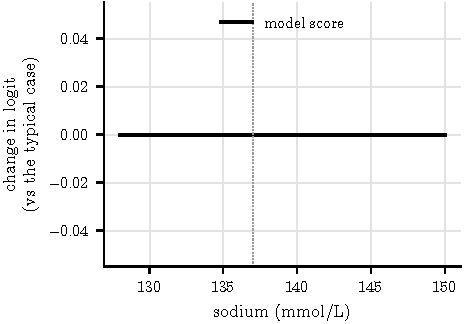
\includegraphics[width=\textwidth,height=0.8\textheight,keepaspectratio]{figures/ch7/options/synthetic-shape-b-sodium}
  \caption{Synthetic data (saddle only), the explained network: response to sodium. Black: the model's score as sodium varies, every other input at the typical case, relative to the typical sodium; dotted: 137 mmol/L. This dataset has no U term.}
  \label{fig:ch7-synthetic-shape-b-sodium}
\end{figure}
